% Supplementary material. Tables are generated by scripts/make_supplement.py from frozen files.
\documentclass[a4paper,11pt]{article}
\usepackage[utf8]{inputenc}
\usepackage[T1]{fontenc}
\usepackage{mathptmx}
\usepackage[margin=2.2cm]{geometry}
\usepackage{amsmath,amssymb}
\usepackage{booktabs,longtable}
\usepackage{graphicx,float}
\usepackage{ragged2e}
\usepackage[hidelinks]{hyperref}
\usepackage{caption}
\captionsetup{font=small,labelfont=bf,justification=raggedright,singlelinecheck=false}
\renewcommand{\thetable}{S\arabic{table}}
\renewcommand{\thefigure}{S\arabic{figure}}
\renewcommand{\thesection}{S\arabic{section}}
\setlength{\LTcapwidth}{\textwidth}
\setlength{\parskip}{4pt}
\setlength{\tabcolsep}{3.5pt}
\setlength{\parindent}{0pt}
\RaggedRight

\title{Supplementary material for\\[2pt]\large Patient-level differential privacy, membership leakage and explanation
fidelity in federated brain tumour MRI classification on a deduplicated benchmark}
\author{Authors to be completed}
\date{}

\begin{document}
\maketitle

\section*{Overview}
This supplement reports every configuration behind the main text, together with the controls and selection steps
that the article summarises in a sentence. All tables were generated by \texttt{scripts/make\_supplement.py} from the
files frozen at repository tag \texttt{v0.9.1-results-frozen}, so each value can be traced to a hashed table or to a
run of a frozen grid. Seeds 1 to 5 give every reported mean, seed 0 serves only for selection, and intervals are
two-sided 95\% $t$ intervals over seeds unless a caption states otherwise.

The sections follow the order of the article. Section S1 documents the duplicate check that defines the clean test
set, Section S2 compares the full and the clean test sets and adds the source controls, Section S3 gives the privacy
accounting and the selection costs, Section S4 covers client count and drift correction, Section S5 adds the
membership-inference detail and Section S6 the explanation detail.

\section{Benchmark curation and near-duplicate check}
Perceptual hashing removed exact and near-exact copies during curation, yet it compares images only in one
orientation. A second check therefore computed the normalised cross-correlation (NCC) between every pair of curated
images at $64\times64$ pixels, once as stored and once with one image mirrored, keeping the larger value. Part A
(Table~\ref{tab:s_ncc}) counts pairs above three thresholds and breaks the cross-split pairs down by the splits they
join.

\begin{table}[H]
\centering\scriptsize
\caption{Part A of the NCC check. Pairs of curated images ($64\times64$) at or above each normalised cross-correlation threshold, taking the larger of the plain and the mirrored comparison.}\label{tab:s_ncc}
\resizebox{\textwidth}{!}{\begin{tabular}{lrrrrrrrr}
\toprule
NCC $\geq$ & Pairs & Same unit & Cross-split & Test--train & Test--val & Train--val & Mirror only & Label conflict \\
\midrule
0.9 & 2296 & 1665 & 295 & 190 & 29 & 76 & 139 & 19 \\
0.95 & 682 & 357 & 148 & 84 & 17 & 47 & 120 & 0 \\
0.98 & 195 & 28 & 80 & 43 & 9 & 28 & 79 & 0 \\
\bottomrule
\end{tabular}}
\end{table}

Across the 813 test images, the NCC to the nearest image in another split has median 0.809, 90th percentile 0.926 and maximum 1.0000. 66 test images reach 0.95 and form the contaminated set.

\begin{table}[H]
\centering\footnotesize
\caption{Part B of the NCC check. Agreement between perceptual-hash duplicates removed during curation and their kept partner, by Hamming distance $d$ of the 64-bit hash.}\label{tab:s_ncc_b}
{\begin{tabular}{lrrrrrr}
\toprule
$d$ & Pairs & Median NCC & Min NCC & $<0.90$ & $<0.95$ & $<0.98$ \\
\midrule
0 & 2945 & 1.0000 & 0.657 & 6 & 10 & 17 \\
2 & 733 & 0.9992 & 0.629 & 13 & 22 & 82 \\
4 & 296 & 0.9735 & 0.558 & 80 & 93 & 176 \\
\bottomrule
\end{tabular}}
\end{table}



At the threshold of 0.95, fixed before the check, 148 pairs crossed a split boundary and 120 of them matched only after
mirroring. Part B (Table~\ref{tab:s_ncc_b}) confirms that the hash and the correlation agree on the duplicates that
curation removed, which shows that the correlation threshold is not looser than the hash it audits.
Figure~\ref{fig:s_montage} shows the most similar cross-split pairs, most of them Br35H no-tumour images whose mirrored
twin sat in another split.

\begin{figure}[!htbp]
\centering
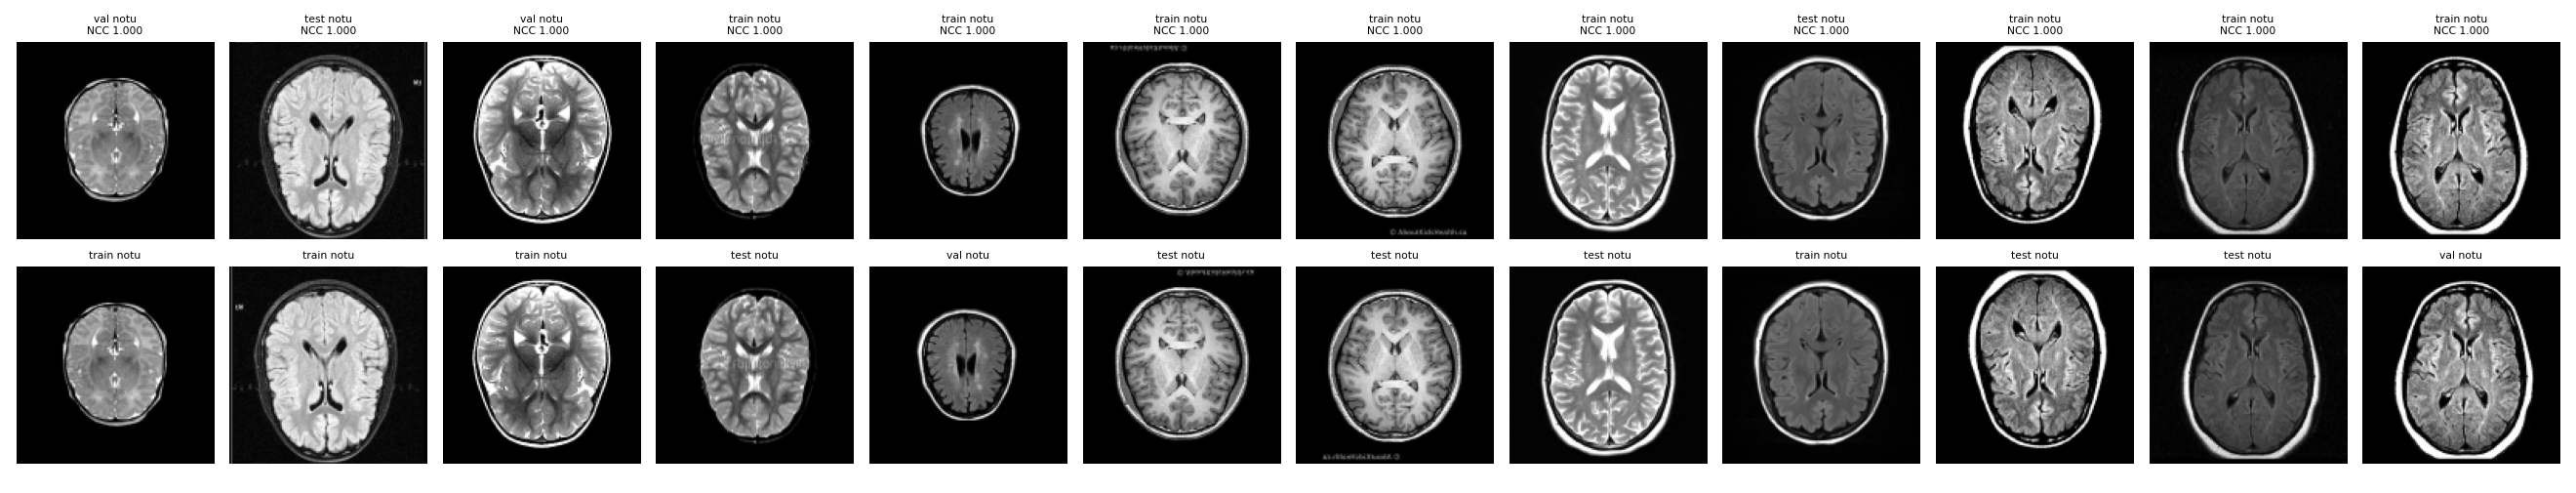
\includegraphics[width=0.92\textwidth]{../../results/ncc/top_cross_split_pairs.png}
\caption{Cross-split pairs with the highest NCC after mirroring. Each pair shows the test image and its nearest image
in another split. These pairs define the 66 contaminated test images excluded from every result in the article.}
\label{fig:s_montage}
\end{figure}

\section{Full and clean test sets, and source controls}
Table~\ref{tab:s_full_clean} lists balanced accuracy for every reported configuration on the full and on the clean
test set. Removing the contaminated images lowered accuracy in every configuration, mostly because no-tumour
sensitivity fell once the mirrored Br35H twins left the test set, yet no ranking between settings changed.

{\scriptsize
\begin{longtable}{llllrrrr}
\caption{Balanced accuracy on the full (813) and clean (747) test sets, mean (95\% CI).}\label{tab:s_full_clean}\\
\toprule
Training & Algorithm & Regime & lr & Bal. acc. (full) & Bal. acc. (clean) & sens$_N$ full & sens$_N$ clean \\
\midrule
\endfirsthead
\toprule
Training & Algorithm & Regime & lr & Bal. acc. (full) & Bal. acc. (clean) & sens$_N$ full & sens$_N$ clean \\
\midrule
\endhead
\bottomrule
\endlastfoot
central & -- & no DP & 0.02 & 0.919 (0.907, 0.931) & 0.908 (0.894, 0.921) & 0.958 & 0.913 \\
central & -- & clip only & 0.02 & 0.871 (0.850, 0.891) & 0.845 (0.818, 0.871) & 0.902 & 0.800 \\
central & -- & $\varepsilon=8$ & 0.02 & 0.815 (0.779, 0.851) & 0.778 (0.739, 0.818) & 0.846 & 0.700 \\
central & -- & $\varepsilon=3$ & 0.02 & 0.686 (0.616, 0.756) & 0.648 (0.572, 0.723) & 0.738 & 0.587 \\
central & -- & $\varepsilon=1$ & 0.02 & 0.331 (0.269, 0.393) & 0.326 (0.272, 0.379) & 0.138 & 0.117 \\
central & -- & patient clip only & 0.02 & 0.884 (0.866, 0.903) & 0.872 (0.852, 0.891) & 0.954 & 0.903 \\
central & -- & patient $\varepsilon=64$ & 0.02 & 0.836 (0.800, 0.873) & 0.820 (0.778, 0.862) & 0.938 & 0.873 \\
central & -- & patient $\varepsilon=32$ & 0.02 & 0.745 (0.698, 0.792) & 0.727 (0.682, 0.771) & 0.922 & 0.850 \\
central & -- & patient $\varepsilon=16$ & 0.02 & 0.584 (0.558, 0.611) & 0.565 (0.543, 0.588) & 0.902 & 0.827 \\
central & -- & patient $\varepsilon=8$ & 0.02 & 0.353 (0.293, 0.413) & 0.337 (0.284, 0.390) & 0.890 & 0.823 \\
central & -- & patient $\varepsilon=3$ & 0.02 & 0.253 (0.245, 0.261) & 0.251 (0.248, 0.253) & 0.992 & 0.983 \\
Dir. 0.1, $K{=}10$ & FedAvg & no DP & 0.01 & 0.843 (0.834, 0.853) & 0.817 (0.806, 0.828) & 0.882 & 0.777 \\
Dir. 0.1, $K{=}10$ & FedAvg & $\varepsilon=8$ & 0.003 & 0.677 (0.632, 0.722) & 0.635 (0.588, 0.682) & 0.614 & 0.447 \\
Dir. 0.1, $K{=}10$ & FedAvg & $\varepsilon=3$ & 0.003 & 0.632 (0.586, 0.678) & 0.589 (0.555, 0.624) & 0.498 & 0.327 \\
Dir. 0.1, $K{=}10$ & FedAvg & $\varepsilon=1$ & 0.003 & 0.322 (0.303, 0.341) & 0.317 (0.301, 0.333) & 0.197 & 0.177 \\
Dir. 0.1, $K{=}10$ & SCAFFOLD & no DP & 0.01 & 0.815 (0.794, 0.836) & 0.790 (0.773, 0.806) & 0.901 & 0.800 \\
Dir. 0.1, $K{=}10$ & SCAFFOLD & $\varepsilon=8$ & 0.003 & 0.705 (0.682, 0.728) & 0.661 (0.632, 0.690) & 0.757 & 0.580 \\
Dir. 0.1, $K{=}10$ & SCAFFOLD & $\varepsilon=3$ & 0.003 & 0.633 (0.571, 0.696) & 0.592 (0.530, 0.653) & 0.549 & 0.383 \\
Dir. 0.5, $K{=}10$ & FedAvg & no DP & 0.01 & 0.878 (0.863, 0.893) & 0.870 (0.852, 0.887) & 0.970 & 0.937 \\
Dir. 0.5, $K{=}10$ & FedAvg & $\varepsilon=8$ & 0.003 & 0.718 (0.686, 0.750) & 0.669 (0.626, 0.712) & 0.771 & 0.577 \\
Dir. 0.5, $K{=}10$ & FedAvg & $\varepsilon=8$ & 0.01 & 0.662 (0.586, 0.739) & 0.624 (0.565, 0.684) & 0.528 & 0.377 \\
Dir. 0.5, $K{=}10$ & FedAvg & $\varepsilon=3$ & 0.003 & 0.626 (0.570, 0.682) & 0.590 (0.548, 0.631) & 0.550 & 0.403 \\
Dir. 0.5, $K{=}10$ & FedAvg & $\varepsilon=1$ & 0.003 & 0.341 (0.286, 0.396) & 0.331 (0.280, 0.383) & 0.326 & 0.287 \\
Dir. 0.5, $K{=}10$ & SCAFFOLD & no DP & 0.01 & 0.889 (0.871, 0.906) & 0.877 (0.857, 0.897) & 0.957 & 0.910 \\
Dir. 0.5, $K{=}10$ & SCAFFOLD & $\varepsilon=8$ & 0.003 & 0.713 (0.681, 0.744) & 0.666 (0.623, 0.708) & 0.784 & 0.597 \\
Dir. 0.5, $K{=}10$ & SCAFFOLD & $\varepsilon=3$ & 0.003 & 0.621 (0.560, 0.682) & 0.582 (0.537, 0.627) & 0.558 & 0.403 \\
Dir. 0.5, $K{=}15$ & FedAvg & no DP & 0.01 & 0.903 (0.897, 0.909) & 0.886 (0.874, 0.899) & 0.938 & 0.870 \\
Dir. 0.5, $K{=}15$ & FedAvg & $\varepsilon=8$ & 0.003 & 0.696 (0.618, 0.774) & 0.655 (0.576, 0.735) & 0.723 & 0.560 \\
Dir. 0.5, $K{=}15$ & FedAvg & $\varepsilon=8$ & 0.01 & 0.564 (0.464, 0.664) & 0.525 (0.449, 0.601) & 0.435 & 0.280 \\
Dir. 0.5, $K{=}15$ & FedAvg & $\varepsilon=3$ & 0.003 & 0.558 (0.458, 0.658) & 0.525 (0.448, 0.602) & 0.398 & 0.267 \\
Dir. 0.5, $K{=}3$ & FedAvg & no DP & 0.01 & 0.868 (0.850, 0.886) & 0.853 (0.827, 0.878) & 0.917 & 0.857 \\
Dir. 0.5, $K{=}3$ & FedAvg & $\varepsilon=8$ & 0.003 & 0.717 (0.644, 0.790) & 0.675 (0.597, 0.754) & 0.693 & 0.527 \\
Dir. 0.5, $K{=}3$ & FedAvg & $\varepsilon=8$ & 0.01 & 0.820 (0.789, 0.852) & 0.779 (0.743, 0.816) & 0.794 & 0.630 \\
Dir. 0.5, $K{=}3$ & FedAvg & $\varepsilon=3$ & 0.003 & 0.719 (0.698, 0.739) & 0.677 (0.644, 0.710) & 0.717 & 0.550 \\
Dir. 0.5, $K{=}5$ & FedAvg & no DP & 0.01 & 0.906 (0.894, 0.919) & 0.892 (0.879, 0.904) & 0.946 & 0.887 \\
Dir. 0.5, $K{=}5$ & FedAvg & $\varepsilon=8$ & 0.003 & 0.735 (0.712, 0.758) & 0.694 (0.667, 0.721) & 0.790 & 0.627 \\
Dir. 0.5, $K{=}5$ & FedAvg & $\varepsilon=8$ & 0.01 & 0.773 (0.713, 0.833) & 0.731 (0.665, 0.798) & 0.779 & 0.613 \\
Dir. 0.5, $K{=}5$ & FedAvg & $\varepsilon=3$ & 0.003 & 0.708 (0.684, 0.732) & 0.669 (0.644, 0.693) & 0.744 & 0.587 \\
Dir. 5.0, $K{=}10$ & FedAvg & no DP & 0.01 & 0.899 (0.878, 0.919) & 0.884 (0.858, 0.909) & 0.946 & 0.887 \\
Dir. 5.0, $K{=}10$ & FedAvg & $\varepsilon=8$ & 0.003 & 0.720 (0.695, 0.745) & 0.674 (0.636, 0.712) & 0.792 & 0.607 \\
Dir. 5.0, $K{=}10$ & FedAvg & $\varepsilon=3$ & 0.003 & 0.623 (0.571, 0.676) & 0.583 (0.542, 0.625) & 0.550 & 0.390 \\
Dir. 5.0, $K{=}10$ & FedAvg & $\varepsilon=1$ & 0.003 & 0.333 (0.280, 0.385) & 0.328 (0.277, 0.379) & 0.266 & 0.247 \\
Dir. 5.0, $K{=}10$ & SCAFFOLD & no DP & 0.01 & 0.907 (0.897, 0.917) & 0.892 (0.879, 0.905) & 0.946 & 0.887 \\
Dir. 5.0, $K{=}10$ & SCAFFOLD & $\varepsilon=8$ & 0.003 & 0.716 (0.692, 0.740) & 0.669 (0.632, 0.705) & 0.789 & 0.600 \\
Dir. 5.0, $K{=}10$ & SCAFFOLD & $\varepsilon=3$ & 0.003 & 0.625 (0.563, 0.686) & 0.585 (0.535, 0.635) & 0.562 & 0.403 \\
IID, $K{=}10$ & FedAvg & no DP & 0.01 & 0.904 (0.893, 0.914) & 0.891 (0.879, 0.904) & 0.954 & 0.903 \\
IID, $K{=}10$ & FedAvg & $\varepsilon=8$ & 0.003 & 0.720 (0.698, 0.742) & 0.673 (0.641, 0.704) & 0.790 & 0.600 \\
IID, $K{=}10$ & FedAvg & $\varepsilon=3$ & 0.003 & 0.639 (0.608, 0.671) & 0.593 (0.558, 0.627) & 0.606 & 0.420 \\
IID, $K{=}10$ & FedAvg & $\varepsilon=1$ & 0.003 & 0.348 (0.311, 0.386) & 0.344 (0.308, 0.380) & 0.304 & 0.287 \\
IID, $K{=}10$ & SCAFFOLD & no DP & 0.01 & 0.909 (0.892, 0.926) & 0.896 (0.878, 0.914) & 0.952 & 0.900 \\
IID, $K{=}10$ & SCAFFOLD & $\varepsilon=8$ & 0.003 & 0.719 (0.699, 0.740) & 0.671 (0.642, 0.701) & 0.789 & 0.597 \\
IID, $K{=}10$ & SCAFFOLD & $\varepsilon=3$ & 0.003 & 0.637 (0.605, 0.668) & 0.589 (0.555, 0.623) & 0.600 & 0.410 \\
natural & FedAvg & no DP & 0.01 & 0.875 (0.868, 0.882) & 0.841 (0.833, 0.848) & 0.824 & 0.687 \\
natural & FedAvg & $\varepsilon=8$ & 0.01 & 0.808 (0.783, 0.833) & 0.765 (0.731, 0.800) & 0.757 & 0.587 \\
natural & FedAvg & $\varepsilon=3$ & 0.003 & 0.714 (0.707, 0.721) & 0.674 (0.659, 0.688) & 0.750 & 0.590 \\
natural & FedAvg & $\varepsilon=1$ & 0.003 & 0.537 (0.474, 0.601) & 0.525 (0.463, 0.586) & 0.366 & 0.317 \\
natural & FedAvg & weight noise $s=0.5$ & 0.01 & 0.259 (0.235, 0.284) & 0.254 (0.243, 0.266) & 0.173 & 0.153 \\
natural & FedAvg & weight noise $s=0.003$ & 0.01 & 0.843 (0.826, 0.860) & 0.801 (0.785, 0.816) & 0.699 & 0.530 \\
natural & FedAvg & patient $\varepsilon=8$ & 0.003 & 0.403 (0.333, 0.472) & 0.398 (0.330, 0.466) & 0.123 & 0.103 \\
natural & SCAFFOLD & no DP & 0.01 & 0.900 (0.889, 0.911) & 0.879 (0.863, 0.895) & 0.920 & 0.837 \\
natural & SCAFFOLD & $\varepsilon=8$ & 0.01 & 0.825 (0.801, 0.849) & 0.790 (0.757, 0.822) & 0.837 & 0.697 \\
natural & SCAFFOLD & $\varepsilon=3$ & 0.003 & 0.713 (0.706, 0.719) & 0.671 (0.661, 0.681) & 0.770 & 0.603 \\
unit Dir. 0.5, $K{=}10$ & FedAvg & patient $\varepsilon=8$ & 0.01 & 0.264 (0.234, 0.294) & 0.271 (0.235, 0.307) & 0.512 & 0.540 \\
\end{longtable}}



Local-only training (Table~\ref{tab:s_local}) shows what each natural client achieves alone. The Br35H client holds no
tumour images and cannot exceed the chance level of 0.25, and even the large Figshare client stays far below the
federated model, so federation adds real value on this partition.

\begin{table}[H]
\centering\footnotesize
\caption{Local-only baselines of the natural partition, seed means.}\label{tab:s_local}
{\begin{tabular}{lrrrr}
\toprule
Client & Regime & Seeds & Bal. acc. (full) & Bal. acc. (clean) \\
\midrule
Br35H & $\varepsilon=8$ & 3 & 0.249 & 0.255 \\
Br35H & no DP & 3 & 0.250 & 0.250 \\
Figshare & $\varepsilon=8$ & 3 & 0.464 & 0.464 \\
Figshare & no DP & 3 & 0.625 & 0.625 \\
SARTAJ & $\varepsilon=8$ & 3 & 0.245 & 0.250 \\
SARTAJ & no DP & 3 & 0.543 & 0.526 \\
\bottomrule
\end{tabular}}
\end{table}



The per-source controls in Table~\ref{tab:s_sources} separate source composition from diagnostic skill. SARTAJ is the
only source with all four classes, and its four-class balanced accuracy stays well below the pooled value in every
setting that learns more than chance, which shows how much the pooled number benefits from sources that hold only one or two classes.

{\scriptsize
\begin{longtable}{lllrrrrrr}
\caption{Per-source controls on the full test set, seed means.}\label{tab:s_sources}\\
\toprule
Mode & Partition & Regime & Bal. acc. & SARTAJ (4 cl.) & Figshare (3 cl.) & Tumour sens. & Spec. SARTAJ & Spec. Br35H \\
\midrule
\endfirsthead
\toprule
Mode & Partition & Regime & Bal. acc. & SARTAJ (4 cl.) & Figshare (3 cl.) & Tumour sens. & Spec. SARTAJ & Spec. Br35H \\
\midrule
\endhead
\bottomrule
\endlastfoot
central & natural & no DP & 0.919 & 0.663 & 0.924 & 0.984 & 0.919 & 0.994 \\
central & natural & clip only & 0.871 & 0.586 & 0.885 & 0.975 & 0.797 & 0.997 \\
central & natural & $\varepsilon=8$ & 0.815 & 0.528 & 0.830 & 0.975 & 0.702 & 0.976 \\
central & natural & $\varepsilon=3$ & 0.686 & 0.467 & 0.681 & 0.958 & 0.590 & 0.870 \\
central & natural & $\varepsilon=1$ & 0.331 & 0.326 & 0.394 & 0.967 & 0.125 & 0.148 \\
central & natural & patient clip only & 0.884 & 0.636 & 0.882 & 0.974 & 0.902 & 1.000 \\
central & natural & patient $\varepsilon=64$ & 0.836 & 0.617 & 0.818 & 0.962 & 0.871 & 0.997 \\
central & natural & patient $\varepsilon=32$ & 0.745 & 0.561 & 0.695 & 0.960 & 0.847 & 0.988 \\
central & natural & patient $\varepsilon=16$ & 0.584 & 0.449 & 0.487 & 0.845 & 0.820 & 0.976 \\
central & natural & patient $\varepsilon=8$ & 0.353 & 0.290 & 0.177 & 0.462 & 0.824 & 0.948 \\
central & natural & patient $\varepsilon=3$ & 0.253 & 0.256 & 0.006 & 0.018 & 0.983 & 1.000 \\
federated & Dir. 0.1, $K{=}10$ & no DP & 0.843 & 0.594 & 0.845 & 0.985 & 0.769 & 0.982 \\
federated & Dir. 0.1, $K{=}10$ & $\varepsilon=8$ & 0.677 & 0.441 & 0.712 & 0.979 & 0.434 & 0.776 \\
federated & Dir. 0.1, $K{=}10$ & $\varepsilon=3$ & 0.632 & 0.429 & 0.690 & 0.972 & 0.342 & 0.636 \\
federated & Dir. 0.1, $K{=}10$ & $\varepsilon=1$ & 0.322 & 0.317 & 0.359 & 0.948 & 0.183 & 0.209 \\
federated & Dir. 0.5, $K{=}10$ & no DP & 0.878 & 0.676 & 0.861 & 0.984 & 0.936 & 1.000 \\
federated & Dir. 0.5, $K{=}10$ & $\varepsilon=8$ & 0.718 & 0.465 & 0.716 & 0.970 & 0.576 & 0.945 \\
federated & Dir. 0.5, $K{=}10$ & $\varepsilon=3$ & 0.626 & 0.434 & 0.662 & 0.973 & 0.397 & 0.688 \\
federated & Dir. 0.5, $K{=}10$ & $\varepsilon=1$ & 0.341 & 0.326 & 0.345 & 0.878 & 0.292 & 0.358 \\
federated & Dir. 5.0, $K{=}10$ & no DP & 0.899 & 0.631 & 0.903 & 0.986 & 0.885 & 1.000 \\
federated & Dir. 5.0, $K{=}10$ & $\varepsilon=8$ & 0.720 & 0.462 & 0.714 & 0.968 & 0.607 & 0.958 \\
federated & Dir. 5.0, $K{=}10$ & $\varepsilon=3$ & 0.623 & 0.428 & 0.658 & 0.975 & 0.393 & 0.691 \\
federated & Dir. 5.0, $K{=}10$ & $\varepsilon=1$ & 0.333 & 0.326 & 0.354 & 0.901 & 0.247 & 0.282 \\
federated & IID, $K{=}10$ & no DP & 0.904 & 0.650 & 0.906 & 0.985 & 0.902 & 1.000 \\
federated & IID, $K{=}10$ & $\varepsilon=8$ & 0.720 & 0.464 & 0.714 & 0.967 & 0.600 & 0.961 \\
federated & IID, $K{=}10$ & $\varepsilon=3$ & 0.639 & 0.432 & 0.661 & 0.967 & 0.427 & 0.767 \\
federated & IID, $K{=}10$ & $\varepsilon=1$ & 0.348 & 0.335 & 0.363 & 0.879 & 0.288 & 0.318 \\
federated & natural & no DP & 0.875 & 0.599 & 0.913 & 0.990 & 0.678 & 0.955 \\
federated & natural & $\varepsilon=8$ & 0.808 & 0.517 & 0.852 & 0.976 & 0.590 & 0.906 \\
federated & natural & $\varepsilon=3$ & 0.714 & 0.498 & 0.716 & 0.977 & 0.593 & 0.891 \\
federated & natural & $\varepsilon=1$ & 0.537 & 0.357 & 0.603 & 0.965 & 0.312 & 0.415 \\
federated & natural & patient $\varepsilon=8$ & 0.403 & 0.312 & 0.503 & 0.967 & 0.092 & 0.152 \\
federated & unit Dir. 0.5, $K{=}10$ & patient $\varepsilon=8$ & 0.264 & 0.255 & 0.184 & 0.497 & 0.549 & 0.479 \\
\end{longtable}}



The probe in Table~\ref{tab:s_probe} asks whether penultimate features reveal the source collection within one class.
Trained models decode source only slightly better than an ImageNet-initialised network and a random network, so the
source signal lives in the images rather than being learned during training.

{\footnotesize
\begin{longtable}{lllrr}
\caption{Source probe on penultimate features, balanced accuracy.}\label{tab:s_probe}\\
\toprule
Mode & Partition & Regime & Tumour probe & No-tumour probe \\
\midrule
\endfirsthead
\toprule
Mode & Partition & Regime & Tumour probe & No-tumour probe \\
\midrule
\endhead
\bottomrule
\endlastfoot
central & natural & no DP & 0.913 (0.888, 0.938) & 0.821 (0.812, 0.831) \\
central & natural & clip only & 0.908 (0.878, 0.938) & 0.808 (0.795, 0.821) \\
central & natural & $\varepsilon=8$ & 0.896 (0.882, 0.909) & 0.794 (0.757, 0.830) \\
central & natural & $\varepsilon=3$ & 0.882 (0.824, 0.941) & 0.770 (0.735, 0.806) \\
central & natural & $\varepsilon=1$ & 0.851 (0.821, 0.882) & 0.769 (0.699, 0.839) \\
central & natural & patient clip only & 0.914 (0.889, 0.939) & 0.813 (0.791, 0.835) \\
central & natural & patient $\varepsilon=64$ & 0.876 (0.857, 0.895) & 0.812 (0.781, 0.843) \\
central & natural & patient $\varepsilon=32$ & 0.864 (0.832, 0.895) & 0.762 (0.730, 0.793) \\
central & natural & patient $\varepsilon=16$ & 0.827 (0.798, 0.855) & 0.780 (0.744, 0.816) \\
central & natural & patient $\varepsilon=8$ & 0.828 (0.784, 0.871) & 0.772 (0.747, 0.797) \\
central & natural & patient $\varepsilon=3$ & 0.794 (0.736, 0.851) & 0.753 (0.699, 0.807) \\
federated & Dir. 0.1, $K{=}10$ & no DP & 0.920 (0.886, 0.955) & 0.827 (0.814, 0.841) \\
federated & Dir. 0.1, $K{=}10$ & $\varepsilon=8$ & 0.895 (0.863, 0.927) & 0.807 (0.790, 0.825) \\
federated & Dir. 0.1, $K{=}10$ & $\varepsilon=3$ & 0.891 (0.862, 0.920) & 0.781 (0.758, 0.805) \\
federated & Dir. 0.1, $K{=}10$ & $\varepsilon=1$ & 0.868 (0.827, 0.909) & 0.812 (0.763, 0.861) \\
federated & Dir. 0.5, $K{=}10$ & no DP & 0.930 (0.919, 0.940) & 0.831 (0.814, 0.849) \\
federated & Dir. 0.5, $K{=}10$ & $\varepsilon=8$ & 0.901 (0.870, 0.932) & 0.813 (0.789, 0.836) \\
federated & Dir. 0.5, $K{=}10$ & $\varepsilon=3$ & 0.891 (0.861, 0.922) & 0.814 (0.765, 0.863) \\
federated & Dir. 0.5, $K{=}10$ & $\varepsilon=1$ & 0.859 (0.821, 0.898) & 0.791 (0.756, 0.826) \\
federated & Dir. 5.0, $K{=}10$ & no DP & 0.921 (0.895, 0.946) & 0.825 (0.804, 0.846) \\
federated & Dir. 5.0, $K{=}10$ & $\varepsilon=8$ & 0.893 (0.875, 0.911) & 0.800 (0.765, 0.834) \\
federated & Dir. 5.0, $K{=}10$ & $\varepsilon=3$ & 0.893 (0.859, 0.926) & 0.813 (0.758, 0.868) \\
federated & Dir. 5.0, $K{=}10$ & $\varepsilon=1$ & 0.872 (0.842, 0.901) & 0.797 (0.764, 0.830) \\
federated & IID, $K{=}10$ & no DP & 0.931 (0.906, 0.955) & 0.839 (0.821, 0.857) \\
federated & IID, $K{=}10$ & $\varepsilon=8$ & 0.897 (0.872, 0.921) & 0.813 (0.781, 0.844) \\
federated & IID, $K{=}10$ & $\varepsilon=3$ & 0.883 (0.859, 0.907) & 0.821 (0.769, 0.873) \\
federated & IID, $K{=}10$ & $\varepsilon=1$ & 0.865 (0.822, 0.909) & 0.775 (0.745, 0.805) \\
federated & natural & no DP & 0.903 (0.890, 0.916) & 0.808 (0.755, 0.861) \\
federated & natural & $\varepsilon=8$ & 0.871 (0.845, 0.898) & 0.811 (0.782, 0.841) \\
federated & natural & $\varepsilon=3$ & 0.875 (0.845, 0.904) & 0.799 (0.776, 0.823) \\
federated & natural & $\varepsilon=1$ & 0.847 (0.809, 0.886) & 0.790 (0.772, 0.807) \\
federated & natural & patient $\varepsilon=8$ & 0.840 (0.782, 0.898) & 0.799 (0.706, 0.892) \\
federated & unit Dir. 0.5, $K{=}10$ & patient $\varepsilon=8$ & 0.822 (0.769, 0.876) & 0.759 (0.727, 0.790) \\
baseline & -- & ImageNet initialisation & 0.871 & 0.783 \\
baseline & -- & random network & 0.846 & 0.776 \\
\end{longtable}}



\section{Privacy accounting and selection cost}
Table~\ref{tab:s_eps} gives the accounted privacy loss of every private configuration. Learning rates for federated
models were chosen among two candidates trained on the same records, and composing the guarantee over both
candidates raises $\varepsilon=8$ to about 12, following the analysis of Papernot and Steinke for hyperparameter
search.

{\scriptsize
\begin{longtable}{lllrrrrr}
\caption{Accounted privacy loss of every private configuration.}\label{tab:s_eps}\\
\toprule
Mode & Partition & Unit & Target $\varepsilon$ & $\sigma$ & $\varepsilon$ & $\varepsilon_{k=2}$ & Worst-unit $\varepsilon$ \\
\midrule
\endfirsthead
\toprule
Mode & Partition & Unit & Target $\varepsilon$ & $\sigma$ & $\varepsilon$ & $\varepsilon_{k=2}$ & Worst-unit $\varepsilon$ \\
\midrule
\endhead
\bottomrule
\endlastfoot
central & natural & image & 1 & 12.885 & 1.00 & -- & -- \\
central & natural & image & 3 & 4.832 & 3.00 & -- & -- \\
central & natural & patient & 3 & 4.832 & 3.00 & -- & 3.00 \\
central & natural & image & 8 & 2.179 & 7.96 & -- & -- \\
central & natural & patient & 8 & 2.179 & 7.96 & -- & 7.96 \\
central & natural & patient & 16 & 1.353 & 15.96 & -- & 15.96 \\
central & natural & patient & 32 & 0.922 & 31.90 & -- & 31.90 \\
central & natural & patient & 64 & 0.673 & 63.69 & -- & 63.69 \\
federated & Dir. 0.1, $K{=}10$ & image & 1 & 12.885 & 1.00 & 1.46 & -- \\
federated & Dir. 0.1, $K{=}10$ & image & 3 & 4.832 & 3.00 & 4.42 & -- \\
federated & Dir. 0.1, $K{=}10$ & image & 8 & 2.179 & 7.96 & 11.98 & -- \\
federated & Dir. 0.5, $K{=}10$ & image & 1 & 12.885 & 1.00 & 1.46 & -- \\
federated & Dir. 0.5, $K{=}10$ & image & 3 & 4.832 & 3.00 & 4.42 & -- \\
federated & Dir. 0.5, $K{=}10$ & image & 8 & 2.179 & 7.96 & 11.98 & -- \\
federated & Dir. 0.5, $K{=}15$ & image & 3 & 4.832 & 3.00 & 4.42 & -- \\
federated & Dir. 0.5, $K{=}15$ & image & 8 & 2.179 & 7.96 & 11.98 & -- \\
federated & Dir. 0.5, $K{=}3$ & image & 3 & 4.832 & 3.00 & 4.42 & -- \\
federated & Dir. 0.5, $K{=}3$ & image & 8 & 2.179 & 7.96 & 11.98 & -- \\
federated & Dir. 0.5, $K{=}5$ & image & 3 & 4.832 & 3.00 & 4.42 & -- \\
federated & Dir. 0.5, $K{=}5$ & image & 8 & 2.179 & 7.96 & 11.98 & -- \\
federated & Dir. 5.0, $K{=}10$ & image & 1 & 12.885 & 1.00 & 1.46 & -- \\
federated & Dir. 5.0, $K{=}10$ & image & 3 & 4.832 & 3.00 & 4.42 & -- \\
federated & Dir. 5.0, $K{=}10$ & image & 8 & 2.179 & 7.96 & 11.98 & -- \\
federated & IID, $K{=}10$ & image & 1 & 12.885 & 1.00 & 1.46 & -- \\
federated & IID, $K{=}10$ & image & 3 & 4.832 & 3.00 & 4.42 & -- \\
federated & IID, $K{=}10$ & image & 8 & 2.179 & 7.96 & 11.98 & -- \\
federated & natural & image & 1 & 12.885 & 1.00 & 1.46 & -- \\
federated & natural & image & 3 & 4.832 & 3.00 & 4.42 & -- \\
federated & natural & image & 8 & 2.179 & 7.96 & 11.98 & -- \\
federated & natural & patient & 8 & 2.179 & 7.96 & 18.39 & 11.98 \\
federated & unit Dir. 0.5, $K{=}10$ & image & 3 & 4.832 & 3.00 & 4.42 & -- \\
federated & unit Dir. 0.5, $K{=}10$ & image & 8 & 2.179 & 7.96 & 11.98 & -- \\
federated & unit Dir. 0.5, $K{=}10$ & patient & 8 & 2.179 & 7.96 & 11.98 & 7.96 \\
\end{longtable}}
\par\smallskip{\footnotesize Central models use the learning rate 0.02 fixed in pilot runs on the same training data, so their selection cost is disclosed but not composed. Natural3 splits 11 units across two clients, which raises the worst-unit guarantee of that partition.}



Table~\ref{tab:s_lr} lists the learning-rate candidates at seed 0 and the one selected by lowest validation loss.
Every non-private configuration selected 0.01, while private ones mostly selected 0.003, which reflects the smaller
steps that noisy gradients tolerate.

{\footnotesize
\begin{longtable}{llrrrc}
\caption{Learning-rate selection at seed 0, federated models.}\label{tab:s_lr}\\
\toprule
Partition & Regime & lr & Best val. loss & Val. bal. acc. & Selected \\
\midrule
\endfirsthead
\toprule
Partition & Regime & lr & Best val. loss & Val. bal. acc. & Selected \\
\midrule
\endhead
\bottomrule
\endlastfoot
natural & no DP & 0.003 & 0.447 & 0.801 &  \\
natural & no DP & 0.01 & 0.333 & 0.847 & \checkmark \\
IID, $K{=}10$ & no DP & 0.003 & 0.310 & 0.882 &  \\
IID, $K{=}10$ & no DP & 0.01 & 0.255 & 0.911 & \checkmark \\
Dir. 0.1, $K{=}10$ & no DP & 0.003 & 0.542 & 0.720 &  \\
Dir. 0.1, $K{=}10$ & no DP & 0.01 & 0.378 & 0.838 & \checkmark \\
Dir. 0.5, $K{=}10$ & no DP & 0.003 & 0.356 & 0.836 &  \\
Dir. 0.5, $K{=}10$ & no DP & 0.01 & 0.318 & 0.889 & \checkmark \\
Dir. 5.0, $K{=}10$ & no DP & 0.003 & 0.309 & 0.875 &  \\
Dir. 5.0, $K{=}10$ & no DP & 0.01 & 0.267 & 0.896 & \checkmark \\
natural & $\varepsilon=8$ & 0.003 & 0.780 & 0.678 &  \\
natural & $\varepsilon=8$ & 0.01 & 0.656 & 0.811 & \checkmark \\
IID, $K{=}10$ & $\varepsilon=8$ & 0.003 & 0.784 & 0.691 & \checkmark \\
IID, $K{=}10$ & $\varepsilon=8$ & 0.01 & 0.823 & 0.648 &  \\
Dir. 0.1, $K{=}10$ & $\varepsilon=8$ & 0.003 & 0.751 & 0.689 & \checkmark \\
Dir. 0.1, $K{=}10$ & $\varepsilon=8$ & 0.01 & 0.901 & 0.568 &  \\
Dir. 0.5, $K{=}10$ & $\varepsilon=8$ & 0.003 & 0.763 & 0.692 & \checkmark \\
Dir. 0.5, $K{=}10$ & $\varepsilon=8$ & 0.01 & 0.877 & 0.644 &  \\
Dir. 5.0, $K{=}10$ & $\varepsilon=8$ & 0.003 & 0.779 & 0.685 & \checkmark \\
Dir. 5.0, $K{=}10$ & $\varepsilon=8$ & 0.01 & 0.835 & 0.625 &  \\
natural & $\varepsilon=3$ & 0.003 & 0.784 & 0.663 & \checkmark \\
natural & $\varepsilon=3$ & 0.01 & 0.812 & 0.588 &  \\
IID, $K{=}10$ & $\varepsilon=3$ & 0.003 & 0.928 & 0.504 & \checkmark \\
IID, $K{=}10$ & $\varepsilon=3$ & 0.01 & 1.228 & 0.336 &  \\
Dir. 0.1, $K{=}10$ & $\varepsilon=3$ & 0.003 & 0.957 & 0.521 & \checkmark \\
Dir. 0.1, $K{=}10$ & $\varepsilon=3$ & 0.01 & 1.241 & 0.299 &  \\
Dir. 0.5, $K{=}10$ & $\varepsilon=3$ & 0.003 & 0.970 & 0.560 & \checkmark \\
Dir. 0.5, $K{=}10$ & $\varepsilon=3$ & 0.01 & 1.255 & 0.299 &  \\
Dir. 5.0, $K{=}10$ & $\varepsilon=3$ & 0.003 & 0.953 & 0.483 & \checkmark \\
Dir. 5.0, $K{=}10$ & $\varepsilon=3$ & 0.01 & 1.233 & 0.308 &  \\
natural & $\varepsilon=1$ & 0.003 & 0.980 & 0.518 & \checkmark \\
natural & $\varepsilon=1$ & 0.01 & 1.363 & 0.274 &  \\
IID, $K{=}10$ & $\varepsilon=1$ & 0.003 & 1.307 & 0.389 & \checkmark \\
IID, $K{=}10$ & $\varepsilon=1$ & 0.01 & 1.769 & 0.275 &  \\
Dir. 0.1, $K{=}10$ & $\varepsilon=1$ & 0.003 & 1.243 & 0.372 & \checkmark \\
Dir. 0.1, $K{=}10$ & $\varepsilon=1$ & 0.01 & 1.889 & 0.251 &  \\
Dir. 0.5, $K{=}10$ & $\varepsilon=1$ & 0.003 & 1.311 & 0.384 & \checkmark \\
Dir. 0.5, $K{=}10$ & $\varepsilon=1$ & 0.01 & 1.738 & 0.269 &  \\
Dir. 5.0, $K{=}10$ & $\varepsilon=1$ & 0.003 & 1.311 & 0.380 & \checkmark \\
Dir. 5.0, $K{=}10$ & $\varepsilon=1$ & 0.01 & 1.693 & 0.276 &  \\
natural & patient $\varepsilon=8$ & 0.003 & 1.191 & 0.408 & \checkmark \\
natural & patient $\varepsilon=8$ & 0.01 & 1.543 & 0.280 &  \\
unit Dir. 0.5, $K{=}10$ & patient $\varepsilon=8$ & 0.003 & 2.098 & 0.353 &  \\
unit Dir. 0.5, $K{=}10$ & patient $\varepsilon=8$ & 0.01 & 2.051 & 0.246 & \checkmark \\
natural & patient $\varepsilon=3$ & 0.003 & 1.410 & 0.267 & \checkmark \\
natural & patient $\varepsilon=3$ & 0.01 & 15.649 & 0.281 &  \\
unit Dir. 0.5, $K{=}10$ & patient $\varepsilon=3$ & 0.003 & 2.275 & 0.214 & \checkmark \\
unit Dir. 0.5, $K{=}10$ & patient $\varepsilon=3$ & 0.01 & 15.845 & 0.250 &  \\
unit Dir. 0.5, $K{=}10$ & no DP & 0.003 & 0.385 & 0.843 &  \\
unit Dir. 0.5, $K{=}10$ & no DP & 0.01 & 0.306 & 0.886 & \checkmark \\
unit Dir. 0.5, $K{=}10$ & $\varepsilon=8$ & 0.003 & 0.783 & 0.681 & \checkmark \\
unit Dir. 0.5, $K{=}10$ & $\varepsilon=8$ & 0.01 & 0.911 & 0.520 &  \\
unit Dir. 0.5, $K{=}10$ & $\varepsilon=3$ & 0.003 & 0.958 & 0.599 & \checkmark \\
unit Dir. 0.5, $K{=}10$ & $\varepsilon=3$ & 0.01 & 1.292 & 0.322 &  \\
\end{longtable}}



\section{Client count and drift correction}
Table~\ref{tab:s_h5} holds the client-count experiment at the shared learning rate of 0.003. The aggregated noise
standard deviation grows with $\sqrt{K}$ at a fixed noise multiplier, and accuracy at $\varepsilon=3$ falls as it
grows, whereas accuracy without privacy shows no trend.

\begin{table}[H]
\centering\footnotesize
\caption{Client count at fixed data, Dirichlet $\alpha=0.5$ FedAvg at learning rate 0.003, full test set. The aggregated noise standard deviation is $\sigma C\sqrt{K}/(qN)$ with $N=2610$.}\label{tab:s_h5}
{\begin{tabular}{rlrrrrr}
\toprule
$K$ & Regime & Client size min/med./max & $\sigma$ & Agg. noise s.d. & Bal. acc. & sens$_M$ \\
\midrule
3 & $\varepsilon=3$ & 424/618/1568 & 4.832 & 0.0321 & 0.719 (0.698, 0.739) & 0.315 \\
5 & $\varepsilon=3$ & 204/452/1065 & 4.832 & 0.0414 & 0.708 (0.684, 0.732) & 0.171 \\
10 & $\varepsilon=3$ & 82/225/533 & 4.832 & 0.0585 & 0.626 (0.570, 0.682) & 0.067 \\
15 & $\varepsilon=3$ & 29/190/354 & 4.832 & 0.0717 & 0.558 (0.458, 0.658) & 0.030 \\
3 & $\varepsilon=8$ & 424/618/1568 & 2.179 & 0.0145 & 0.717 (0.644, 0.790) & 0.305 \\
5 & $\varepsilon=8$ & 204/452/1065 & 2.179 & 0.0187 & 0.735 (0.712, 0.758) & 0.244 \\
10 & $\varepsilon=8$ & 82/225/533 & 2.179 & 0.0264 & 0.718 (0.686, 0.750) & 0.193 \\
15 & $\varepsilon=8$ & 29/190/354 & 2.179 & 0.0323 & 0.696 (0.618, 0.774) & 0.163 \\
3 & no DP & 424/618/1568 & 0.000 & 0.0000 & 0.868 (0.850, 0.886) & 0.643 \\
5 & no DP & 204/452/1065 & 0.000 & 0.0000 & 0.906 (0.894, 0.919) & 0.811 \\
10 & no DP & 82/225/533 & 0.000 & 0.0000 & 0.878 (0.863, 0.893) & 0.605 \\
15 & no DP & 29/190/354 & 0.000 & 0.0000 & 0.903 (0.897, 0.909) & 0.799 \\
\bottomrule
\end{tabular}}
\end{table}



FedProx screening at seed 0 (Table~\ref{tab:s_fedprox}) shows that proximal weights up to 0.1 change validation loss
only in the third decimal place. Larger weights helped in a few private settings and hurt elsewhere, without a
consistent pattern that would justify carrying FedProx to the seed runs.

{\scriptsize
\begin{longtable}{lllrrrrr}
\caption{FedProx screening at seed 0. Best validation loss of FedAvg ($\mu=0$) and of FedProx with proximal weight $\mu$, at the learning rate selected for FedAvg.}\label{tab:s_fedprox}\\
\toprule
Partition & Regime & lr & $\mu=0$ & $\mu=0.01$ & $\mu=0.1$ & $\mu=1$ & $\mu=10$ \\
\midrule
\endfirsthead
\toprule
Partition & Regime & lr & $\mu=0$ & $\mu=0.01$ & $\mu=0.1$ & $\mu=1$ & $\mu=10$ \\
\midrule
\endhead
\bottomrule
\endlastfoot
Dir. 0.1, $K{=}10$ & $\varepsilon=3$ & 0.003 & 0.957 & 0.957 & 0.954 & 0.944 & 0.930 \\
Dir. 0.1, $K{=}10$ & $\varepsilon=8$ & 0.003 & 0.751 & 0.751 & 0.751 & 0.751 & 0.770 \\
Dir. 0.1, $K{=}10$ & no DP & 0.01 & 0.378 & 0.374 & 0.378 & 0.405 & 0.570 \\
Dir. 0.5, $K{=}10$ & $\varepsilon=3$ & 0.003 & 0.970 & 0.970 & 0.969 & 0.962 & 0.906 \\
Dir. 0.5, $K{=}10$ & $\varepsilon=8$ & 0.003 & 0.763 & 0.763 & 0.764 & 0.767 & 0.812 \\
Dir. 0.5, $K{=}10$ & no DP & 0.01 & 0.318 & 0.318 & 0.317 & 0.323 & 0.339 \\
Dir. 5.0, $K{=}10$ & $\varepsilon=3$ & 0.003 & 0.953 & 0.953 & 0.952 & 0.942 & 0.911 \\
Dir. 5.0, $K{=}10$ & $\varepsilon=8$ & 0.003 & 0.779 & 0.779 & 0.779 & 0.783 & 0.819 \\
Dir. 5.0, $K{=}10$ & no DP & 0.01 & 0.267 & 0.267 & 0.266 & 0.266 & 0.300 \\
IID, $K{=}10$ & $\varepsilon=3$ & 0.003 & 0.928 & 0.928 & 0.928 & 0.924 & 0.900 \\
IID, $K{=}10$ & $\varepsilon=8$ & 0.003 & 0.784 & 0.784 & 0.784 & 0.786 & 0.823 \\
IID, $K{=}10$ & no DP & 0.01 & 0.255 & 0.255 & 0.254 & 0.262 & 0.290 \\
natural3 & $\varepsilon=3$ & 0.003 & 0.784 & 0.784 & 0.785 & 0.789 & 0.838 \\
natural3 & $\varepsilon=8$ & 0.01 & 0.656 & 0.658 & 0.656 & 0.665 & 0.734 \\
natural3 & no DP & 0.01 & 0.333 & 0.340 & 0.343 & 0.371 & 0.516 \\
\end{longtable}}



Table~\ref{tab:s_scaffold} compares size-weighted SCAFFOLD with FedAvg. No difference survives Holm correction, and the
uniform server average of the original algorithm collapses on unequal clients under privacy, most visibly on natural3,
where one client holds 78\% of the images.

\begin{table}[H]
\centering\scriptsize
\caption{SCAFFOLD against FedAvg, full test set. Size-weighted SCAFFOLD over seeds 1 to 5 with paired $t$-tests and Holm correction, and the uniform server average over seeds 1 to 3.}\label{tab:s_scaffold}
\resizebox{\textwidth}{!}{\begin{tabular}{llrrrrrr}
\toprule
Partition & Regime & FedAvg & SCAFFOLD (size) & Diff. & $p$ & $p$ Holm & SCAFFOLD (uniform) \\
\midrule
natural & no DP & 0.875 & 0.900 & +0.025 & 0.0043 & 0.064 & 0.898 \\
Dir. 5.0, $K{=}10$ & $\varepsilon=8$ & 0.720 & 0.716 & -0.004 & 0.0054 & 0.075 & 0.713 \\
Dir. 0.1, $K{=}10$ & no DP & 0.843 & 0.815 & -0.028 & 0.0132 & 0.172 & 0.761 \\
natural & $\varepsilon=8$ & 0.808 & 0.825 & +0.017 & 0.0136 & 0.172 & 0.590 \\
Dir. 0.5, $K{=}10$ & no DP & 0.878 & 0.889 & +0.011 & 0.0514 & 0.566 & 0.886 \\
Dir. 0.1, $K{=}10$ & $\varepsilon=8$ & 0.677 & 0.705 & +0.028 & 0.1132 & 1.000 & 0.428 \\
IID, $K{=}10$ & no DP & 0.904 & 0.909 & +0.005 & 0.2159 & 1.000 & 0.904 \\
IID, $K{=}10$ & $\varepsilon=3$ & 0.639 & 0.637 & -0.003 & 0.2306 & 1.000 & 0.642 \\
Dir. 0.5, $K{=}10$ & $\varepsilon=3$ & 0.626 & 0.621 & -0.006 & 0.3204 & 1.000 & 0.492 \\
Dir. 5.0, $K{=}10$ & no DP & 0.898 & 0.907 & +0.008 & 0.3871 & 1.000 & 0.903 \\
Dir. 0.5, $K{=}10$ & $\varepsilon=8$ & 0.718 & 0.713 & -0.005 & 0.4677 & 1.000 & 0.718 \\
IID, $K{=}10$ & $\varepsilon=8$ & 0.720 & 0.719 & -0.001 & 0.5066 & 1.000 & 0.728 \\
natural & $\varepsilon=3$ & 0.714 & 0.713 & -0.001 & 0.7524 & 1.000 & 0.358 \\
Dir. 5.0, $K{=}10$ & $\varepsilon=3$ & 0.623 & 0.625 & +0.001 & 0.8260 & 1.000 & 0.642 \\
Dir. 0.1, $K{=}10$ & $\varepsilon=3$ & 0.632 & 0.633 & +0.001 & 0.9456 & 1.000 & 0.268 \\
\bottomrule
\end{tabular}}
\end{table}



\section{Membership inference}
The weight-noise comparator used a rule fixed before any seed run. Table~\ref{tab:s_wn} shows that the literal
$s=0.5$ of the prior study diverged, and the rule selected $s=0.003$ as the largest level whose validation loss did not
exceed that of record-level $\varepsilon=8$.

\begin{table}[H]
\centering\footnotesize
\caption{Selection of the utility-matched weight-noise level at seed 0 on natural3. Gaussian noise $\mathcal{N}(0,s^2)$ is added to each client's weights after local training, without clipping.}\label{tab:s_wn}
{\begin{tabular}{rrrr}
\toprule
$s$ & Diverged & Best val. loss & Meets reference \\
\midrule
0.5 & yes & 21.214 & no \\
0.05 & no & 15.452 & no \\
0.01 & no & 0.945 & no \\
0.003 & no & 0.357 & yes \\
0.001 & no & 0.313 & yes \\
\bottomrule
\end{tabular}}
\par\smallskip{\footnotesize The reference is the seed-0 validation loss of record-level $\varepsilon=8$ FedAvg on natural3, 0.656. The rule takes the largest $s$ that meets it. Over seeds 1 to 5 on the full test set, weight noise $s=0.5$ reaches balanced accuracy 0.259 (0.235, 0.284) and weight noise $s=0.003$ reaches balanced accuracy 0.843 (0.826, 0.860).}
\end{table}



Tables~\ref{tab:s_week07_clean_lira} and \ref{tab:s_week07_lira} report LiRA with the clean and with the full test set
as non-members, in both its online and its offline form. The choice of non-member set changes no conclusion, since
online AUC, true-positive rate at 1\% false positives and patient AUC move by less than 0.01 for every target that
produced a usable model, and every private setting stays at the level of a random guess under both definitions.

\begin{table}[H]
\centering\scriptsize
\caption{LiRA against natural3 FedAvg with 16 shadow models, clean test set (747 images) as non-members. Online and offline variants, mean over target seeds with 95\% $t$ interval.}\label{tab:s_week07_clean_lira}
\resizebox{\textwidth}{!}{\begin{tabular}{lrrrrrrrr}
\toprule
Target & $n$ & AUC & TPR@1\% & TPR@0.1\% & Patient AUC & Off. AUC & Off. TPR@1\% & Off. patient AUC \\
\midrule
no DP & 5 & 0.666 (0.642, 0.689) & 0.108 (0.081, 0.135) & 0.033 (0.019, 0.046) & 0.805 (0.762, 0.848) & 0.656 & 0.068 & 0.769 \\
$\varepsilon=8$ & 5 & 0.464 (0.448, 0.480) & 0.017 (0.012, 0.022) & 0.006 (0.003, 0.008) & 0.454 (0.427, 0.481) & 0.503 & 0.016 & 0.511 \\
$\varepsilon=3$ & 5 & 0.545 (0.522, 0.567) & 0.015 (0.008, 0.023) & 0.003 (0.002, 0.005) & 0.567 (0.529, 0.605) & 0.546 & 0.014 & 0.581 \\
$\varepsilon=1$ & 5 & 0.479 (0.469, 0.489) & 0.010 (0.006, 0.015) & 0.003 (0.000, 0.005) & 0.457 (0.413, 0.500) & 0.488 & 0.012 & 0.500 \\
weight noise $s=0.5$ & 5 & 0.474 (0.437, 0.511) & 0.038 (0.023, 0.053) & 0.003 (0.002, 0.003) & 0.518 (0.497, 0.539) & 0.538 & 0.034 & 0.545 \\
weight noise $s=0.003$ & 5 & 0.594 (0.572, 0.616) & 0.045 (0.038, 0.051) & 0.016 (0.012, 0.020) & 0.745 (0.713, 0.778) & 0.569 & 0.030 & 0.665 \\
\bottomrule
\end{tabular}}
\end{table}

\begin{table}[H]
\centering\scriptsize
\caption{LiRA against natural3 FedAvg with 16 shadow models, full test set (813 images) as non-members. Online and offline variants, mean over target seeds with 95\% $t$ interval.}\label{tab:s_week07_lira}
\resizebox{\textwidth}{!}{\begin{tabular}{lrrrrrrrr}
\toprule
Target & $n$ & AUC & TPR@1\% & TPR@0.1\% & Patient AUC & Off. AUC & Off. TPR@1\% & Off. patient AUC \\
\midrule
no DP & 5 & 0.662 (0.642, 0.682) & 0.112 (0.084, 0.140) & 0.033 (0.019, 0.046) & 0.805 (0.762, 0.848) & 0.661 & 0.069 & 0.769 \\
$\varepsilon=8$ & 5 & 0.472 (0.459, 0.484) & 0.015 (0.010, 0.020) & 0.002 (-0.000, 0.005) & 0.454 (0.427, 0.481) & 0.497 & 0.013 & 0.511 \\
$\varepsilon=3$ & 5 & 0.545 (0.524, 0.565) & 0.017 (0.010, 0.023) & 0.003 (0.002, 0.005) & 0.567 (0.529, 0.604) & 0.546 & 0.014 & 0.581 \\
$\varepsilon=1$ & 5 & 0.483 (0.473, 0.493) & 0.009 (0.005, 0.013) & 0.001 (-0.000, 0.002) & 0.456 (0.412, 0.500) & 0.489 & 0.010 & 0.499 \\
weight noise $s=0.5$ & 5 & 0.480 (0.455, 0.504) & 0.022 (0.014, 0.030) & 0.003 (0.002, 0.003) & 0.518 (0.497, 0.538) & 0.529 & 0.024 & 0.545 \\
weight noise $s=0.003$ & 5 & 0.589 (0.568, 0.610) & 0.047 (0.038, 0.055) & 0.016 (0.012, 0.020) & 0.745 (0.714, 0.777) & 0.585 & 0.033 & 0.665 \\
\bottomrule
\end{tabular}}
\end{table}



The loss-threshold attack in Table~\ref{tab:s_loss_mia} is far weaker than LiRA even without privacy. Its values below
0.5 under privacy persist when the attack is computed within each source and class stratum, so they do not arise from
the mix of sources and classes in each split.

{\scriptsize
\begin{longtable}{lllrrrrr}
\caption{Loss-threshold membership attack, AUC.}\label{tab:s_loss_mia}\\
\toprule
Mode & Partition & Regime & Pooled (full) & Stratum (full) & Pooled (clean) & Stratum (clean) & Figshare (clean) \\
\midrule
\endfirsthead
\toprule
Mode & Partition & Regime & Pooled (full) & Stratum (full) & Pooled (clean) & Stratum (clean) & Figshare (clean) \\
\midrule
\endhead
\bottomrule
\endlastfoot
central & natural & no DP & 0.540 & 0.531 & 0.550 & 0.533 & 0.540 \\
central & natural & clip only & 0.494 & 0.479 & 0.510 & 0.478 & 0.488 \\
central & natural & $\varepsilon=8$ & 0.485 & 0.466 & 0.497 & 0.465 & 0.477 \\
central & natural & $\varepsilon=3$ & 0.493 & 0.474 & 0.499 & 0.474 & 0.492 \\
central & natural & $\varepsilon=1$ & 0.513 & 0.500 & 0.498 & 0.499 & 0.517 \\
central & natural & patient $\varepsilon=8$ & 0.511 & 0.507 & 0.546 & 0.507 & 0.505 \\
central & natural & patient $\varepsilon=3$ & 0.506 & 0.502 & 0.543 & 0.502 & 0.499 \\
central & natural & patient clip only & 0.505 & 0.477 & 0.539 & 0.477 & 0.482 \\
central & natural & patient $\varepsilon=16$ & 0.495 & 0.478 & 0.529 & 0.477 & 0.481 \\
central & natural & patient $\varepsilon=32$ & 0.501 & 0.481 & 0.536 & 0.481 & 0.488 \\
central & natural & patient $\varepsilon=64$ & 0.495 & 0.471 & 0.529 & 0.470 & 0.472 \\
federated & Dir. 0.1, $K{=}10$ & $\varepsilon=1$ & 0.505 & 0.503 & 0.496 & 0.503 & 0.514 \\
federated & Dir. 0.1, $K{=}10$ & $\varepsilon=3$ & 0.493 & 0.480 & 0.485 & 0.480 & 0.491 \\
federated & Dir. 0.1, $K{=}10$ & $\varepsilon=8$ & 0.496 & 0.482 & 0.494 & 0.482 & 0.495 \\
federated & Dir. 0.1, $K{=}10$ & no DP & 0.518 & 0.506 & 0.527 & 0.506 & 0.515 \\
federated & Dir. 0.5, $K{=}10$ & $\varepsilon=1$ & 0.508 & 0.496 & 0.504 & 0.496 & 0.515 \\
federated & Dir. 0.5, $K{=}10$ & $\varepsilon=3$ & 0.501 & 0.491 & 0.495 & 0.491 & 0.502 \\
federated & Dir. 0.5, $K{=}10$ & $\varepsilon=8$ & 0.496 & 0.483 & 0.501 & 0.482 & 0.495 \\
federated & Dir. 0.5, $K{=}10$ & no DP & 0.526 & 0.518 & 0.548 & 0.519 & 0.521 \\
federated & Dir. 5.0, $K{=}10$ & $\varepsilon=1$ & 0.507 & 0.496 & 0.499 & 0.496 & 0.515 \\
federated & Dir. 5.0, $K{=}10$ & $\varepsilon=3$ & 0.501 & 0.491 & 0.495 & 0.491 & 0.502 \\
federated & Dir. 5.0, $K{=}10$ & $\varepsilon=8$ & 0.495 & 0.479 & 0.501 & 0.479 & 0.492 \\
federated & Dir. 5.0, $K{=}10$ & no DP & 0.526 & 0.521 & 0.537 & 0.522 & 0.526 \\
federated & IID, $K{=}10$ & $\varepsilon=1$ & 0.507 & 0.493 & 0.502 & 0.493 & 0.515 \\
federated & IID, $K{=}10$ & $\varepsilon=3$ & 0.498 & 0.486 & 0.495 & 0.487 & 0.500 \\
federated & IID, $K{=}10$ & $\varepsilon=8$ & 0.495 & 0.479 & 0.501 & 0.479 & 0.493 \\
federated & IID, $K{=}10$ & no DP & 0.532 & 0.528 & 0.546 & 0.529 & 0.533 \\
federated & natural & $\varepsilon=1$ & 0.497 & 0.475 & 0.487 & 0.474 & 0.498 \\
federated & natural & $\varepsilon=3$ & 0.490 & 0.473 & 0.491 & 0.472 & 0.487 \\
federated & natural & $\varepsilon=8$ & 0.476 & 0.459 & 0.478 & 0.458 & 0.470 \\
federated & natural & no DP & 0.532 & 0.526 & 0.521 & 0.527 & 0.535 \\
federated & natural & patient $\varepsilon=8$ & 0.499 & 0.489 & 0.477 & 0.488 & 0.502 \\
federated & unit Dir. 0.5, $K{=}10$ & patient $\varepsilon=8$ & 0.497 & 0.498 & 0.519 & 0.496 & 0.488 \\
federated & natural & weight noise $s=0.5$ & 0.506 & 0.497 & 0.487 & 0.497 & 0.514 \\
federated & natural & weight noise $s=0.003$ & 0.505 & 0.498 & 0.488 & 0.499 & 0.504 \\
\end{longtable}}



\section{Explanations}
Table~\ref{tab:s_xai} reports localisation and faithfulness for Grad-CAM, Grad-CAM++ and Integrated Gradients across
the privacy settings of central training. Grad-CAM shows the clearest decline as the privacy budget shrinks,
Grad-CAM++ declines more gently, and Integrated Gradients reaches the highest pointing rate without privacy, a result
that the randomisation check below qualifies.

{\footnotesize
\begin{longtable}{llrrrrr}
\caption{Localisation and faithfulness of three attribution methods for central models on correctly classified Figshare test tumour images with expert masks, seed means. Lower deletion and higher insertion AUC indicate more faithful maps.}\label{tab:s_xai}\\
\toprule
Regime & Method & Pointing & IoU top 15\% & Energy in mask & Deletion & Insertion \\
\midrule
\endfirsthead
\toprule
Regime & Method & Pointing & IoU top 15\% & Energy in mask & Deletion & Insertion \\
\midrule
\endhead
\bottomrule
\endlastfoot
no DP & Grad-CAM & 0.197 & 0.087 & 0.032 & 0.290 & 0.604 \\
no DP & Grad-CAM++ & 0.139 & 0.080 & 0.032 & 0.310 & 0.585 \\
no DP & Int. Gradients & 0.276 & 0.058 & 0.065 & 0.151 & 0.462 \\
clip only & Grad-CAM & 0.190 & 0.086 & 0.031 & 0.382 & 0.689 \\
clip only & Grad-CAM++ & 0.152 & 0.084 & 0.032 & 0.389 & 0.676 \\
clip only & Int. Gradients & 0.200 & 0.054 & 0.057 & 0.214 & 0.479 \\
$\varepsilon=8$ & Grad-CAM & 0.156 & 0.076 & 0.029 & 0.406 & 0.715 \\
$\varepsilon=8$ & Grad-CAM++ & 0.129 & 0.079 & 0.030 & 0.429 & 0.705 \\
$\varepsilon=8$ & Int. Gradients & 0.198 & 0.051 & 0.053 & 0.311 & 0.510 \\
$\varepsilon=3$ & Grad-CAM & 0.103 & 0.055 & 0.027 & 0.490 & 0.688 \\
$\varepsilon=3$ & Grad-CAM++ & 0.098 & 0.069 & 0.028 & 0.494 & 0.708 \\
$\varepsilon=3$ & Int. Gradients & 0.172 & 0.046 & 0.048 & 0.353 & 0.531 \\
$\varepsilon=1$ & Grad-CAM & 0.089 & 0.032 & 0.027 & 0.480 & 0.526 \\
$\varepsilon=1$ & Grad-CAM++ & 0.123 & 0.065 & 0.031 & 0.469 & 0.546 \\
$\varepsilon=1$ & Int. Gradients & 0.123 & 0.047 & 0.049 & 0.469 & 0.595 \\
patient clip only & Grad-CAM & 0.187 & 0.085 & 0.032 & 0.307 & 0.620 \\
patient clip only & Grad-CAM++ & 0.115 & 0.077 & 0.032 & 0.330 & 0.590 \\
patient clip only & Int. Gradients & 0.239 & 0.055 & 0.060 & 0.155 & 0.396 \\
patient $\varepsilon=64$ & Grad-CAM & 0.127 & 0.058 & 0.029 & 0.290 & 0.555 \\
patient $\varepsilon=64$ & Grad-CAM++ & 0.147 & 0.079 & 0.031 & 0.285 & 0.568 \\
patient $\varepsilon=64$ & Int. Gradients & 0.193 & 0.052 & 0.054 & 0.103 & 0.363 \\
patient $\varepsilon=32$ & Grad-CAM & 0.097 & 0.042 & 0.027 & 0.267 & 0.459 \\
patient $\varepsilon=32$ & Grad-CAM++ & 0.129 & 0.075 & 0.029 & 0.251 & 0.521 \\
patient $\varepsilon=32$ & Int. Gradients & 0.168 & 0.047 & 0.048 & 0.102 & 0.322 \\
patient $\varepsilon=16$ & Grad-CAM & 0.069 & 0.032 & 0.025 & 0.269 & 0.375 \\
patient $\varepsilon=16$ & Grad-CAM++ & 0.111 & 0.063 & 0.028 & 0.252 & 0.433 \\
patient $\varepsilon=16$ & Int. Gradients & 0.147 & 0.046 & 0.047 & 0.105 & 0.247 \\
patient $\varepsilon=8$ & Grad-CAM & 0.082 & 0.029 & 0.025 & 0.276 & 0.314 \\
patient $\varepsilon=8$ & Grad-CAM++ & 0.102 & 0.047 & 0.028 & 0.238 & 0.363 \\
patient $\varepsilon=8$ & Int. Gradients & 0.206 & 0.049 & 0.051 & 0.163 & 0.248 \\
patient $\varepsilon=3$ & Grad-CAM & 0.056 & 0.023 & 0.018 & 0.345 & 0.300 \\
patient $\varepsilon=3$ & Grad-CAM++ & 0.000 & 0.030 & 0.018 & 0.281 & 0.334 \\
patient $\varepsilon=3$ & Int. Gradients & 0.000 & 0.039 & 0.039 & 0.272 & 0.162 \\
\end{longtable}}



The randomisation check in Table~\ref{tab:s_rand} decides which method deserves interpretation. Integrated Gradients
with a black baseline keeps a rank correlation near 0.7 with maps from a network whose weights were all re-initialised,
so its maps mostly reflect the input rather than the learned model, whereas Grad-CAM correlations stay between $-0.05$
and $0.39$.

\begin{table}[H]
\centering\footnotesize
\caption{Model-parameter randomisation check, Spearman rank correlation between maps of the trained model and of a fully re-initialised network (central models, seed 1). Values near zero pass the check. All layers re-initialises every weight, last block only the final residual block and the classifier.}\label{tab:s_rand}
{\begin{tabular}{lrrrr}
\toprule
Regime & Grad-CAM, all layers & Grad-CAM, last block & IG, all layers & IG, last block \\
\midrule
no DP & 0.310 & 0.444 & 0.684 & 0.709 \\
clip only & 0.328 & 0.408 & 0.700 & 0.709 \\
$\varepsilon=8$ & 0.388 & 0.377 & 0.706 & 0.714 \\
$\varepsilon=3$ & 0.324 & 0.029 & 0.699 & 0.722 \\
$\varepsilon=1$ & -0.047 & 0.309 & 0.703 & 0.728 \\
patient clip only & 0.166 & 0.477 & 0.683 & 0.705 \\
patient $\varepsilon=64$ & 0.232 & 0.491 & 0.694 & 0.719 \\
patient $\varepsilon=32$ & 0.309 & 0.403 & 0.703 & 0.726 \\
patient $\varepsilon=16$ & 0.035 & -0.010 & 0.690 & 0.710 \\
patient $\varepsilon=8$ & 0.050 & 0.316 & 0.698 & 0.726 \\
patient $\varepsilon=3$ & 0.101 & 0.098 & 0.712 & 0.731 \\
\bottomrule
\end{tabular}}
\end{table}



Table~\ref{tab:s_border} tests for skull-border and background artefacts, adds Grad-CAM from the third residual block at
twice the resolution and lists the cross-seed consistency used in the article. Grad-CAM places less mass on the brain rim
and outside the brain than their area shares, so neither artefact explains the localisation results.

{\scriptsize
\begin{longtable}{lllrrrrrrr}
\caption{Border-rim analysis, layer-3 Grad-CAM ($8\times8$) and cross-seed consistency. Rim and outside-brain values are the share of Grad-CAM mass, next to the share of image area (chance).}\label{tab:s_border}\\
\toprule
Mode & Partition & Regime & Rim & Rim chance & Outside & Outside chance & L3 pointing & L3 IoU & Consistency \\
\midrule
\endfirsthead
\toprule
Mode & Partition & Regime & Rim & Rim chance & Outside & Outside chance & L3 pointing & L3 IoU & Consistency \\
\midrule
\endhead
\bottomrule
\endlastfoot
central & natural3 & no DP & 0.175 & 0.334 & 0.261 & 0.405 & 0.192 & 0.055 & 0.700 \\
central & natural3 & clip only & 0.174 & 0.334 & 0.266 & 0.401 & 0.142 & 0.043 & 0.663 \\
central & natural3 & $\varepsilon=8$ & 0.176 & 0.334 & 0.280 & 0.398 & 0.123 & 0.044 & 0.485 \\
central & natural3 & $\varepsilon=3$ & 0.180 & 0.333 & 0.294 & 0.389 & 0.103 & 0.038 & 0.309 \\
central & natural3 & $\varepsilon=1$ & 0.180 & 0.351 & 0.362 & 0.443 & 0.051 & 0.027 & 0.235 \\
central & natural3 & patient $\varepsilon=8$ & 0.180 & 0.332 & 0.333 & 0.417 & 0.060 & 0.028 & 0.218 \\
central & natural3 & patient $\varepsilon=3$ & 0.176 & 0.308 & 0.289 & 0.329 & 0.056 & 0.009 & 0.234 \\
central & natural3 & patient clip only & 0.175 & 0.335 & 0.280 & 0.405 & 0.145 & 0.048 & 0.609 \\
central & natural3 & patient $\varepsilon=16$ & 0.181 & 0.335 & 0.318 & 0.406 & 0.066 & 0.030 & 0.225 \\
central & natural3 & patient $\varepsilon=32$ & 0.176 & 0.332 & 0.296 & 0.395 & 0.113 & 0.040 & 0.291 \\
central & natural3 & patient $\varepsilon=64$ & 0.174 & 0.332 & 0.299 & 0.399 & 0.156 & 0.049 & 0.368 \\
federated & Dir. 0.1, $K{=}10$ & $\varepsilon=1$ & 0.163 & 0.358 & 0.406 & 0.452 & 0.056 & 0.024 & 0.291 \\
federated & Dir. 0.1, $K{=}10$ & $\varepsilon=3$ & 0.176 & 0.335 & 0.290 & 0.395 & 0.045 & 0.021 & 0.364 \\
federated & Dir. 0.1, $K{=}10$ & $\varepsilon=8$ & 0.174 & 0.334 & 0.274 & 0.395 & 0.120 & 0.037 & 0.489 \\
federated & Dir. 0.1, $K{=}10$ & no DP & 0.173 & 0.334 & 0.269 & 0.399 & 0.101 & 0.037 & 0.687 \\
federated & Dir. 0.5, $K{=}10$ & $\varepsilon=1$ & 0.193 & 0.359 & 0.407 & 0.462 & 0.051 & 0.026 & 0.302 \\
federated & Dir. 0.5, $K{=}10$ & $\varepsilon=3$ & 0.176 & 0.331 & 0.258 & 0.383 & 0.082 & 0.035 & 0.451 \\
federated & Dir. 0.5, $K{=}10$ & $\varepsilon=8$ & 0.173 & 0.333 & 0.258 & 0.390 & 0.131 & 0.043 & 0.513 \\
federated & Dir. 0.5, $K{=}10$ & no DP & 0.174 & 0.335 & 0.261 & 0.401 & 0.161 & 0.049 & 0.725 \\
federated & Dir. 5.0, $K{=}10$ & $\varepsilon=1$ & 0.188 & 0.359 & 0.406 & 0.458 & 0.049 & 0.022 & 0.312 \\
federated & Dir. 5.0, $K{=}10$ & $\varepsilon=3$ & 0.176 & 0.330 & 0.258 & 0.382 & 0.088 & 0.034 & 0.456 \\
federated & Dir. 5.0, $K{=}10$ & $\varepsilon=8$ & 0.173 & 0.333 & 0.255 & 0.389 & 0.141 & 0.043 & 0.523 \\
federated & Dir. 5.0, $K{=}10$ & no DP & 0.173 & 0.335 & 0.264 & 0.404 & 0.157 & 0.048 & 0.703 \\
federated & IID, $K{=}10$ & $\varepsilon=1$ & 0.192 & 0.360 & 0.416 & 0.462 & 0.048 & 0.022 & 0.303 \\
federated & IID, $K{=}10$ & $\varepsilon=3$ & 0.175 & 0.330 & 0.251 & 0.381 & 0.089 & 0.038 & 0.476 \\
federated & IID, $K{=}10$ & $\varepsilon=8$ & 0.173 & 0.332 & 0.254 & 0.388 & 0.140 & 0.043 & 0.526 \\
federated & IID, $K{=}10$ & no DP & 0.173 & 0.334 & 0.262 & 0.403 & 0.155 & 0.048 & 0.705 \\
federated & natural3 & $\varepsilon=1$ & 0.174 & 0.335 & 0.287 & 0.401 & 0.074 & 0.032 & 0.356 \\
federated & natural3 & $\varepsilon=3$ & 0.175 & 0.331 & 0.251 & 0.386 & 0.124 & 0.044 & 0.532 \\
federated & natural3 & $\varepsilon=8$ & 0.175 & 0.333 & 0.280 & 0.399 & 0.118 & 0.041 & 0.467 \\
federated & natural3 & no DP & 0.174 & 0.335 & 0.267 & 0.405 & 0.118 & 0.041 & 0.657 \\
\end{longtable}}



\section*{Open questions and risks}
\begin{enumerate}
\item The patient-level guarantee is exact only for Figshare, because SARTAJ and Br35H units are groups of similar
images rather than verified patients, and some of those groups may still combine different people.
\item Mirrored pairs remain between training and validation data (47 pairs at NCC 0.95), so round and learning-rate
selection drew on slightly contaminated validation data even though every test result excludes contaminated images.
\item Central models use a learning rate fixed in pilot runs on the same training data, and this selection cost is
disclosed rather than composed into $\varepsilon$.
\item The H5 mechanism table, the SCAFFOLD comparison and the source controls are computed on the full test set,
and the clean-set versions of the corresponding main-text values come from Table~\ref{tab:s_full_clean}.
\item Randomisation was checked on one seed per setting with 64 images, which suffices to separate the two methods but
not to rank privacy settings against each other.
\end{enumerate}

\end{document}
